\documentclass[12pt]{article}
\usepackage{amsmath}
\usepackage[lmargin = 1in, rmargin = 1in, tmargin = 1in, bmargin = 1in]{geometry}
\usepackage[none]{hyphenat}
\usepackage{graphicx}
\usepackage{subcaption}
\usepackage{float}

\title{\textbf{Problem 5\\Generalized Reduced Gradient Method}}
\author{Aditya Vipradas\\ASU ID: 1209435588}
\begin{document}
\maketitle
The given optimization problem with two equality constraints is solved using the GRG method in MATLAB. The initial guess for x1, x2 and x3 is taken to be 0.7, 0.5 and 0.6 respectively. The Levenberg-Marquardt method is implemented to remove singularity observed in the matrices. The stopping criterion tolerance for the reduced gradient is considered to be 0.001. For the given problem, the minimum is obtained at (x1, x2, x3) = (-1.5445, 1.4195, -0.12499) and the corresponding function value is 4.4161 as observed in the following plot where the red star mark denotes the minimum. The function value logarithmic error plot is also shown below.
\begin{figure}[H]
\begin{center}
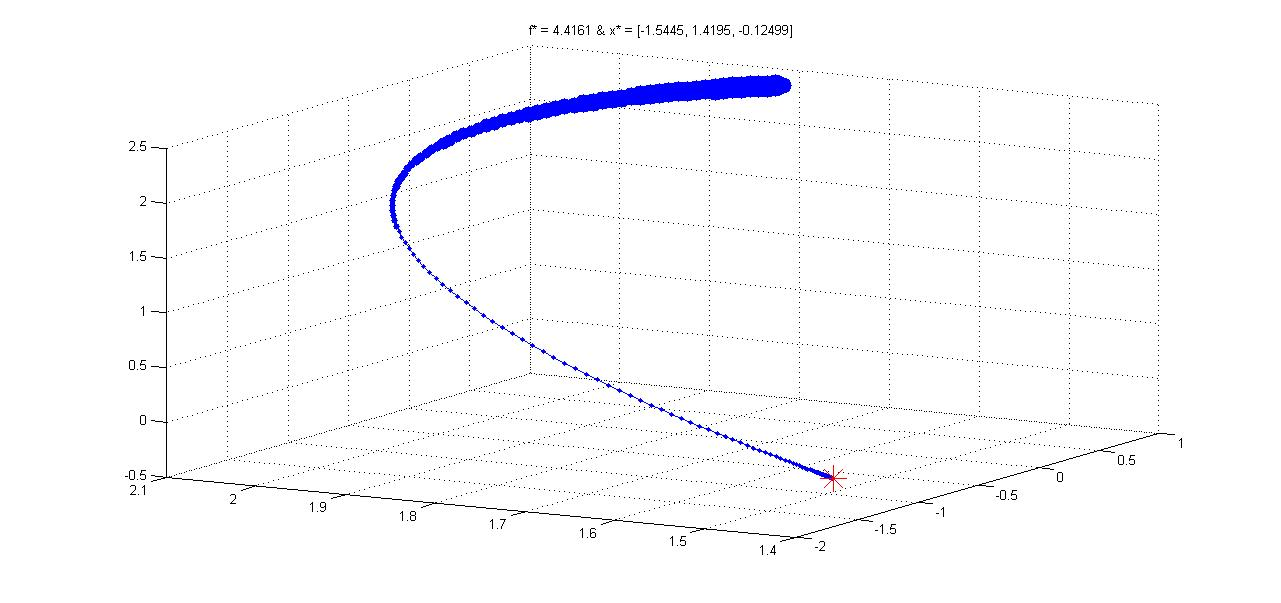
\includegraphics[scale=0.4]{2.jpg}
\caption{Minimum (red star) obtained from GRG method}  
\end{center}
\end{figure}
\begin{figure}[H]
\begin{center}
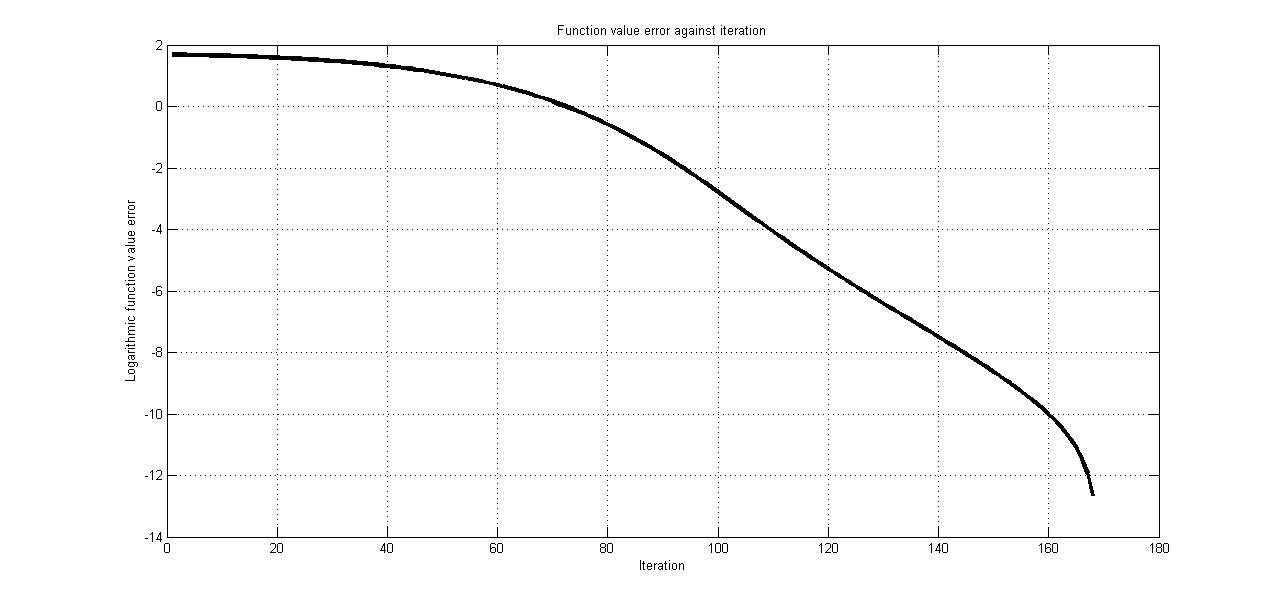
\includegraphics[scale=0.4]{1.jpg}
\caption{Function error plot}  
\end{center}
\end{figure}
\end{document}
Refer the following slides for the primary MATLAB code.